\section{Developer Biography}\label{chap:biography}
\vspace{-0.9em}
\begin{figure}[!htpb]
\centering
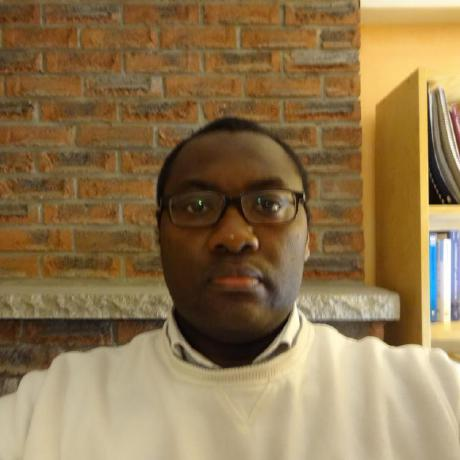
\includegraphics[scale=0.35]{../../francais/images/XavierNOUNDOU-2}
\caption{Portrait of Xavier}~\label{fig:xaviernoumbis}
\end{figure}

\company{Xavier NOUMBISSI NOUNDOU} is a Cameroonian,
and was born in $1983$.
He holds a Master's degree in Computer Science
(\emph{Diplom--Informatiker} [\emph{\diplinf}]) of
the \textbf{\unibremen} in Germany.

During his \diplinf--studies at the \unibremen, Xavier worked
part--time, for $25$ months, as, Software Developer for
\textbf{\bergmann}, located in Hamburg, at Rellingen, in Germany.

Xavier worked as Junior Software Developer for 21 months
at \company{\siemens} (Erlangen, Germany) just after
obtaining his Master's degree in Computer Science.

Xavier leaves ''\siemens'' in July~$2009$ to pursue doctoral
studies (Ph.D. in Software~Engineering) in the area of research
''static code--analysis'' in the research laboratory
\company{Watform} of the \company{University of Waterloo}.

In $2012$, Xavier worked~$8$ months as a Ph.D.--graduate intern
at \company{IBM Toronto Lab} in Markham (Ontario, Canada).
Xavier was in the JIT compilation team of \emph{Java J~$9$}.

In March~$2015$, Xavier leaves the research laboratory ''Watform'',
to found the computer system startup--company \company{\yerenlabs}.

Xavier reads, writes, and talks fluently in English,
French, and German.
